\documentclass[11pt]{scrartcl}
\usepackage[sexy]{{style_files/evan}}

\usepackage{{style_files/NMC}}
\usepackage{standalone}
\usepackage{import}

\begin{document}
\title{NMC Problem Set \#20} % add # of pset
\date{Jan. 1, 2023} % add date
\maketitle

\section*{Welcome!}

This is a selection of interesting problems derived from curious thoughts, curated so you can nibble on them throughout the week! The point of this document is to introduce you to fun puzzles that require thinking. We recommend you try the ones that you find interesting! Feel free to work on them with others (even us teachers!). Harder problems are marked with chilies (\fullchili), in case you want to challenge yourself.
\newline\newline
Have fun! \textit{Note: New variants on these problems may be released throughout the week. Remember to check back once in a while!}
    
\section{Algebra}
\begin{enumerate}[label=\textbf{A\arabic*}.]
    \item \textbf{Fruit Swap} \newline
    A fruit vendor sells apples and oranges, of which they are sorted into $3$ labeled crates. Suppose one crate has apples only, another crate has oranges only, and the third has an even mix of apples and oranges, of which all $3$ are incorrectly labeled (i.e. the crate with only apples might have been mislabeled as a mixed crate).

    \begin{enumerate}
        \item You are allowed to pick one fruit at random from one crate. Is it possible to relabel all $3$ crates correctly? \footnote{for the record, no, you don't get to grope the fruits to see if there are oranges and/or apples in the crate. nuh-uh.}

        \item (\halfchili) Suppose we now have $7$ distinct but mislabeled crates with $3$ kinds of fruits. $3$ of the crates contain only one kind of fruit, another $3$ of the crates contain two kinds of fruits and the last crate contains a mix of the three. If you are only allowed to pick one fruit out of each crate, how many crates do you have to go through before being able to determine which crate contains what?
    \end{enumerate}
    
\end{enumerate}

\newpage
\section{Combinatorics}
\begin{enumerate}[label=\textbf{C\arabic*}.]
    \item (\halfchili) \textbf{Rerolling Dice} \newline
    We have two $6$-sided dice, each labeled $1$ to $6$ on its faces. Suppose we roll them both and record the sum of the rolls, before repeating the procedure again (reroll). What is the expected value of the larger sum between both rolls?

    \item \textbf{Cleanup} \newline
    In an act of rebellion, an obstinate kid has a tantrum and chucks $n$ balls into $k$ empty bins at random. What's the expected number of empty bins? \footnote{assume the kid is michael jordan and they dont miss when throwing the balls into bins.}
    
\end{enumerate}

\newpage
\section{Geometry}
\begin{enumerate}[label=\textbf{G\arabic*}.]
    \item \textbf{Lance was Here} \newline
    Suppose we have a triangle $ABC$ with altitudes $BE$ and $CF$. Two circles pass through $A$ and $F$ such that they are both tangent to $BC$ in distinct points $P$ and $Q$. Prove that the intersection of $PE$ and $QF$ lies on the circumcircle of $AEF$.

    \begin{figure}[h]
        \centering
        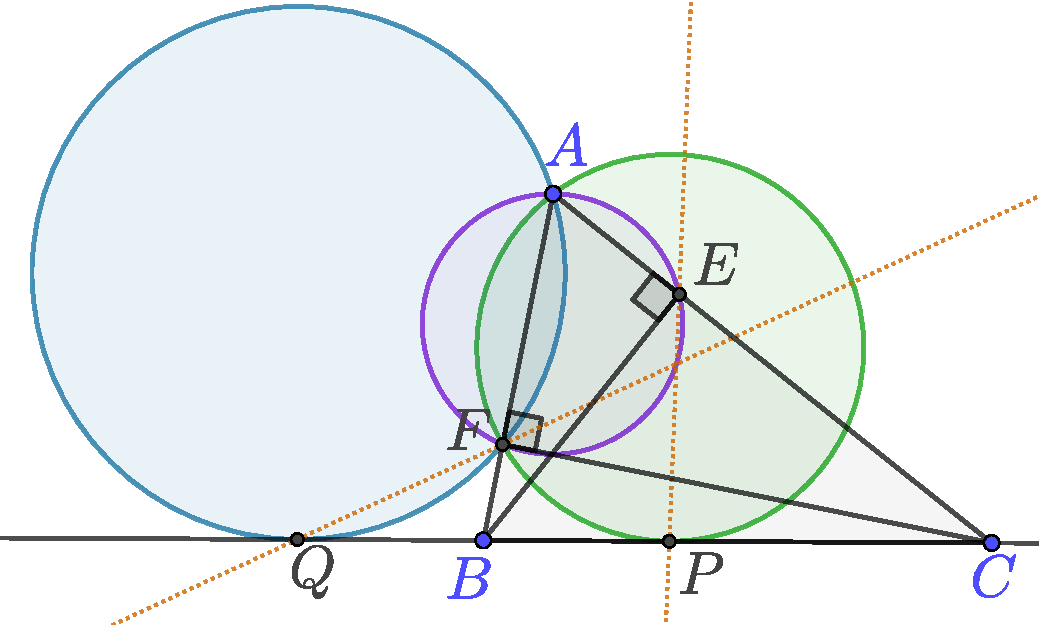
\includegraphics[width = 12cm]{weekly/week 20/Diagrams/lancegeow20.pdf} % 15cm = aligned?
        \caption{Sample Diagram from Lance. Wasn't able to convert this into TikZ :(}
        \label{fig:lancewashere}
    \end{figure} 
\end{enumerate}

\newpage
\section{Number Theory}
\begin{enumerate}[label=\textbf{N\arabic*}.]
    \item (\fullchili) \textbf{Digit Sums} \newline
    Denote $S(x)$ as the sum of the digits of $x$ when written in base $10$. Prove that $S(2^n) > S(2^{n+1})$ for infinitely many positive integers $n$.

    \item (\fullchili) \textbf{Trigonometry is Funky} \newline
    Let $(a_k)$ correspond to the integers in the set $\{ 1, 2, \dots, n \}$ that are relatively prime to $n$. For which $n$ is the following true?
    \[ \left\lvert \, \prod_{i=1}^k \cos\left( \frac{\pi a_i}{n} \right) \right\rvert = 2^{-\varphi(n)}. \]
\end{enumerate}

\end{document}
